% Created 2016-08-10 Wed 13:52
\documentclass[presentation]{beamer}
\usepackage[utf8]{inputenc}
\usepackage[T1]{fontenc}
\usepackage{fixltx2e}
\usepackage{graphicx}
\usepackage{grffile}
\usepackage{longtable}
\usepackage{wrapfig}
\usepackage{rotating}
\usepackage[normalem]{ulem}
\usepackage{amsmath}
\usepackage{textcomp}
\usepackage{amssymb}
\usepackage{capt-of}
\usepackage{hyperref}
\usetheme{Madrid}
\author{Mario Raul Freitas}
\date{\today}
\title{Curso de Python - Dia 3}
\hypersetup{
 pdfauthor={Mario Raul Freitas},
 pdftitle={Curso de Python - Dia 3},
 pdfkeywords={},
 pdfsubject={},
 pdfcreator={Emacs 25.0.94.2 (Org mode 8.3.5)}, 
 pdflang={English}}
\begin{document}

\maketitle

\section{GUI}
\label{sec:orgheadline2}
\begin{frame}[label={sec:orgheadline1}]{Main Window Vs Parent Widget Vs Child Widget}
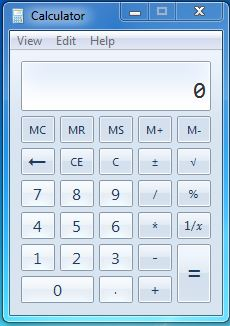
\includegraphics[width=.9\linewidth]{img/GUI/Calculadora_2016-08-04_21-43-00.JPG}
\end{frame}
\section{PyQt}
\label{sec:orgheadline13}
\begin{frame}[label={sec:orgheadline3}]{Sobre o PyQt}
Uma das melhores ferramentas para criar GUIs em Python

Multiplataforma entre Windows, Linux e Mac

Simples e intuitivo
\end{frame}
\begin{frame}[fragile,label={sec:orgheadline4}]{Imports}
 \begin{verbatim}
from PyQt4 import QtGui
import sys
\end{verbatim}
\end{frame}
\begin{frame}[fragile,label={sec:orgheadline5}]{Main Function}
 \begin{verbatim}
def main():
    app = QtGui.QApplication(sys.argv)
    GUI = MainWindow()
    sys.exit(app.exec_())

main()
\end{verbatim}
\end{frame}
\begin{frame}[fragile,label={sec:orgheadline6}]{Class MainWindow}
 \begin{verbatim}
class MainWindow(QtGui.QMainWindow):
    def __init__(self, parent=None):
        super(MainWindow, self).__init__(parent)

        self.show()
\end{verbatim}
\end{frame}
\begin{frame}[fragile,label={sec:orgheadline7}]{MainWindow Parameters}
 \begin{verbatim}
# Dentro do __init__ de MainWindow
self.setGeometry(100, 100, 300, 400)
self.setWindowTitle('Calculadora')
self.setWindowIcon(QtGui.QIcon('icon_64.png'))
\end{verbatim}
\end{frame}
\begin{frame}[fragile,label={sec:orgheadline8}]{MainWidget}
 \begin{verbatim}
# Dentro do __init__ de MainWindow
mainWidget = MainWidget(self)
self.setCentralWidget(mainWidget)
\end{verbatim}
\end{frame}
\begin{frame}[fragile,label={sec:orgheadline9}]{Class MainWidget}
 \begin{verbatim}
class MainWidget(QtGui.QWidget):
    def __init__(self, parent):
        super(MainWidget, self).__init__(parent)
\end{verbatim}
\end{frame}
\begin{frame}[fragile,label={sec:orgheadline10}]{Child Widgets}
 \begin{verbatim}
# Dentro do __init__ de MainWidget
self.lb1 = QtGui.QLabel('Eu sou um texto', self)
self.le1 = QtGui.QLineEdit(self)
self.te1 = QtGui.QTextEdit(self)
self.rbt1 = QtGui.QRadioButton('Option 1', self)
self.cbt1 = QtGui.QCheckBox('C1', self)
self.bt1 = QtGui.QPushButton('Sair', self)

self.cbox = QtGui.QComboBox(self)
self.cbox.addItem('Op1')
self.cbox.addItem('Op2')

self.lbl1.move(30, 50)
\end{verbatim}
\end{frame}
\begin{frame}[fragile,label={sec:orgheadline11}]{Layout}
 \begin{verbatim}
# Dentro do __init__ de MainWidget
layout = QtGui.QGridLayout()

layout.addWidget(self.lb1, 1, 1)
layout.addWidget(self.cbox, 1, 2)
layout.addWidget(self.bt1, 2, 1, 1, 2)

self.setLayout(layout)
\end{verbatim}
\end{frame}
\begin{frame}[fragile,label={sec:orgheadline12}]{Connect Button}
 \begin{verbatim}
    # Dentro do __init__ da MainWidget
    self.bt1.clicked.connect(self.exit_gui)

def exit_gui(self):
        sys.exit()
\end{verbatim}
\end{frame}
\section{Calculadora}
\label{sec:orgheadline17}
Vamos utilizar os conhecimentos adquiridos para construir uma calculadora capaz de realizar contas simples.
\begin{frame}[fragile,label={sec:orgheadline14}]{Calculadora - Objetos}
 \begin{verbatim}
# Dentro do __init__ de MainWidget
self.lb1 = QtGui.QLabel('Primeiro Numero: ', self)
self.lb2 = QtGui.QLabel('Segundo Numero: ', self)
self.lb3 = QtGui.QLabel('Resultado: ', self)
        
self.bt1 = QtGui.QPushButton('+', self)
self.bt2 = QtGui.QPushButton('-', self)
self.bt3 = QtGui.QPushButton('X', self)
self.bt4 = QtGui.QPushButton('/', self)
        
self.le1 = QtGui.QLineEdit(self)
self.le2 = QtGui.QLineEdit(self)
self.le3 = QtGui.QLineEdit(self)
\end{verbatim}
\end{frame}
\begin{frame}[fragile,label={sec:orgheadline15}]{Calculadora - Layout}
 \begin{verbatim}
# Dentro do __init__ de MainWidget
layout = QtGui.QGridLayout()
        
layout.addWidget(self.lb1, 1, 1, 1, 2)
layout.addWidget(self.le1, 1, 3, 1, 2)
layout.addWidget(self.lb2, 2, 1, 1, 2)
layout.addWidget(self.le2, 2, 3, 1, 2)
layout.addWidget(self.bt1, 3, 1)
layout.addWidget(self.bt2, 3, 2)
layout.addWidget(self.bt3, 3, 3)
layout.addWidget(self.bt4, 3, 4)
layout.addWidget(self.lb3, 4, 1, 1, 2)
layout.addWidget(self.le3, 4, 3, 1, 2)
        
self.setLayout(layout)
\end{verbatim}
\end{frame}
\begin{frame}[fragile,label={sec:orgheadline16}]{Calculadora - Connect}
 \begin{verbatim}
    # Dentro do __init__ de MainWidget
    self.bt1.clicked.connect(self.mais)
    self.bt2.clicked.connect(self.menos)
    self.bt3.clicked.connect(self.vezes)
    self.bt4.clicked.connect(self.div)

def mais(self):
    a = float(self.le1.text())
    b = float(self.le2.text())
    self.le3.setText(str(a+b))

def menos(self):
    a = float(self.le1.text())
    b = float(self.le2.text())
    self.le3.setText(str(a-b))

def vezes(self):
    a = float(self.le1.text())
    b = float(self.le2.text())
    self.le3.setText(str(a*b))

def div(self):
    a = float(self.le1.text())
    b = float(self.le2.text())
    self.le3.setText(str(a/b))
\end{verbatim}
\end{frame}
\section{CivCom Diagram Calculator - GUI}
\label{sec:orgheadline29}
\begin{frame}[fragile,label={sec:orgheadline18}]{Imports}
 \begin{verbatim}
from T09_Diagrams import Moment
from PyQt4 import QtGui
import sys
\end{verbatim}
\end{frame}
\begin{frame}[fragile,label={sec:orgheadline19}]{Main Function}
 \begin{verbatim}
def main():
    app = QtGui.QApplication(sys.argv)
    GUI = MainWindow()
    sys.exit(app.exec_())

if __name__ == '__main__':
    main()
\end{verbatim}
\end{frame}
\begin{frame}[fragile,label={sec:orgheadline20}]{MainWindow}
 \begin{verbatim}
class MainWindow(QtGui.QMainWindow): 
    def __init__(self, parent=None):
        super(MainWindow, self).__init__(parent)
        
        mainWidget = MainWidget(self)
        self.setCentralWidget(mainWidget)

        self.setGeometry(100, 100, 300, 400)
        self.setWindowTitle('CivCom Diagram Calculator')
        self.setWindowIcon(QtGui.QIcon('icon_32.png')
 
        self.quit_act()
        self.about_act()
        self.menu_act() 
     
        self.show()
        # self.showMaximized()
        # self.showFullScreen()
\end{verbatim}
\end{frame}
\begin{frame}[fragile,label={sec:orgheadline21}]{Quit Act()}
 \begin{verbatim}
def quit_act(self):
    self.quitAct = QtGui.QAction('Sair', self)
    self.quitAct.setShortcut('Ctrl+Q')
    self.quitAct.setStatusTip('Fecha o programa.')
    self.quitAct.triggered.connect(sys.exit)
\end{verbatim}
\end{frame}
\begin{frame}[fragile,label={sec:orgheadline22}]{About Act()}
 \begin{verbatim}
def about_act(self):
    self.aboutmsg = QtGui.QMessageBox()
    self.aboutmsg.setText('CivCom Diagram Calculator - Version 0.1')
    self.aboutmsg.setInformativeText('Esse programa toma as variaveis de uma viga biengastada ' +
                                  'e do carregamento sobre ela e gera os diagramas de momento ' +
                                  'e deflexao da viga')
    self.aboutmsg.setWindowTitle('CivCom Diagram Calculator')
    self.aboutmsg.setIconPixmap(QtGui.QPixmap('icon_s.jpg')) 
    
    self.aboutAct = QtGui.QAction('Sobre', self)
    self.aboutAct.setShortcut('F1')
    self.aboutAct.setStatusTip('Mostra as informacoes do programa')
    self.aboutAct.triggered.connect(self.aboutmsg.exec_)
\end{verbatim}
\end{frame}
\begin{frame}[fragile,label={sec:orgheadline23}]{Menu Act()}
 \begin{verbatim}
def menu_act(self):
    # Menus Principais
    mainMenu = self.menuBar() 
    fileMenu = mainMenu.addMenu('Arquivo')           
    helpMenu = mainMenu.addMenu('Ajuda')                   
    fileMenu.addAction(self.quitAct)                     
    helpMenu.addAction(self.aboutAct)                  
    self.statusBar()
\end{verbatim}
\end{frame}
\begin{frame}[fragile,label={sec:orgheadline24}]{MainWidget}
 \begin{verbatim}
class MainWidget(QtGui.QWidget):                                                           
    def __init__(self, parent):                                                     
        super(MainWidget, self).__init__(parent)
        
        # Objetos
        # Layout
   
    # Metodos
\end{verbatim}
\end{frame}
\begin{frame}[fragile,label={sec:orgheadline25}]{Objetos}
 \begin{verbatim}
# Dentro de __init__ de MainWidget
self.lbl1 = QtGui.QLabel('Tipo de Carga: ')      

self.dbtn = QtGui.QComboBox(self)
self.dbtn.addItem('Uniforme')  
self.dbtn.addItem('Concentrada')   

self.lbl2 = QtGui.QLabel('Comprimento da Barra (m): ')

self.ledit1 = QtGui.QLineEdit(self) 
self.ledit1.setPlaceholderText('Digite o comprimento da barra aqui.')  

self.lbl3 = QtGui.QLabel('Magnitude do Carregamento (kN ou kN/m): ')

self.ledit2 = QtGui.QLineEdit(self)
self.ledit2.setPlaceholderText('Digite a magnitude do carregamento aqui.')

self.pshbtn1 = QtGui.QPushButton('Plotar Diagrama', self)
self.pshbtn1.clicked.connect(self.calc_diagram)
\end{verbatim}
\end{frame}
\begin{frame}[fragile,label={sec:orgheadline26}]{Layout}
 \begin{verbatim}
# Dentro de __init__ de MainWidget
grid = QtGui.QGridLayout()      
grid.addWidget(self.lbl1, 1, 1)    
grid.addWidget(self.dbtn, 1, 2)     
grid.addWidget(self.lbl2, 2, 1)                                      
grid.addWidget(self.ledit1, 2, 2)                             
grid.addWidget(self.lbl3, 3, 1)                                    
grid.addWidget(self.ledit2, 3, 2)                                    
grid.addWidget(self.pshbtn1, 4, 1, 1, 2)                  
self.setLayout(grid)
\end{verbatim}
\end{frame}
\begin{frame}[fragile,label={sec:orgheadline27}]{Calc Diagram()}
 \begin{verbatim}
def calc_diagram(self):
    ltype = self.dbtn.currentText()       
    length = float(self.ledit1.text())   
    magnitude = float(self.ledit2.text())   
    moment_d = Moment(ltype, length, magnitude)
    moment_d.plot_m_diagram()
\end{verbatim}
\end{frame}
\begin{frame}[label={sec:orgheadline28}]{COMO MELHORAR?}
Outros Carregamentos

Outros Apoios

Calcular Deflexão

Método das Diferenças Finitas

Método dos Elementos Finitos

Método da Rigidez Direta
\end{frame}
\end{document}